\section{Соответствие объём--граница}
Важнейшее свойство топологических изоляторов --- наличие киральных краевых состояний.
Оказывается, что на границе нормального и топологического изоляторов всегда существуют
краевые моды, причём разность числа мод, движущихся в одну сторону, и мод, движущихся в 
противоположную сторону, равна величине $\mathrm{TKNN}$--инварианта. 

Для всех упомянутых выше моделей это утверждение можно проверить, диагонализуя 
численно гамильтониан полосы, имеющей конечную толщину по одной из осей.
На всех полученных спектрах видны уровни, пересекающие запрещённую зону. Именно 
они соответствуют краевым состояниям.

\begin{figure}[h]
    \centering
    \begin{minipage}[b]{0.4\textwidth}
        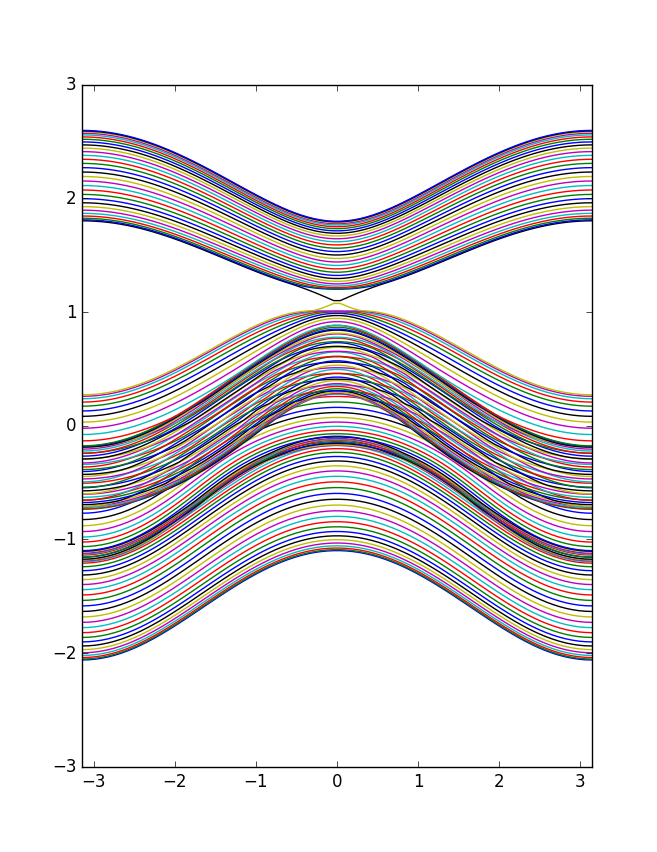
\includegraphics[width=\linewidth]{toy_ham_stripe.png}
    \end{minipage}
    \begin{minipage}[b]{0.4\textwidth}
        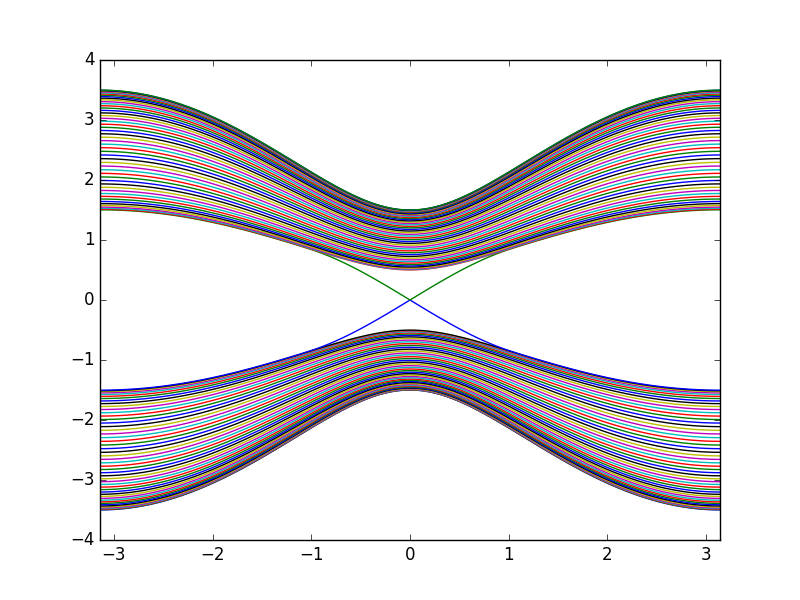
\includegraphics[width=\linewidth]{eff_ham_stripe.png}
    \end{minipage}
\end{figure}
